\documentclass[]{article}

\usepackage[math]{kurier}
\usepackage[sc]{mathpazo}
\renewcommand{\sfdefault}{kurier}

%I added this to the template
\usepackage{float}
\usepackage{amsmath}
\usepackage{graphicx}
\usepackage{amsmath}
\usepackage{graphicx}
\usepackage[colorinlistoftodos]{todonotes}
\usepackage[colorlinks=true, allcolors=blue]{hyperref}
\usepackage{authblk}
\usepackage{tabularx}

\usepackage{graphicx}
\graphicspath{ {imgs/} }

\setlength{\oddsidemargin}{0.25 in}
\setlength{\evensidemargin}{-0.25 in}
\setlength{\topmargin}{-0.6 in}
\setlength{\textwidth}{6.5 in}
\setlength{\textheight}{8.5 in}
\setlength{\headsep}{0.75 in}
\setlength{\parindent}{0 in}
\setlength{\parskip}{0.1 in}


\newcounter{lecnum}
\renewcommand{\thepage}{\thelecnum-\arabic{page}}
\renewcommand{\thesection}{\thelecnum.\arabic{section}}
\renewcommand{\theequation}{\thelecnum.\arabic{equation}}
\renewcommand{\thefigure}{\thelecnum.\arabic{figure}}
\renewcommand{\thetable}{\thelecnum.\arabic{table}}


\newcommand{\lecture}[3]{
   \pagestyle{myheadings}
   \thispagestyle{plain}
   \newpage
   \setcounter{lecnum}{#1}
   \setcounter{page}{1}
   \noindent
   \begin{center}
   \framebox{
      \vbox{\vspace{2mm}
    \hbox to 6.28in { {\bf \sffamily AA 274: Principles of Robotic Autonomy
                        \hfill Winter 2018} }
       \vspace{4mm}
       \hbox to 6.28in { {\sffamily{\Large \hfill Lecture #1: #2  \hfill}} }
       \vspace{2mm}
       % \hbox to 6.28in { {\it \hfill Scribes: #4} }
      \vspace{2mm}}
   }
   \end{center}
   \markboth{Lecture #1: #2}{Lecture #1: #2}

   \vspace*{4mm}
}

%%%%%%%%%%%%%%%%%%%%%%%%%%
%document
\begin{document}
%modify this
\lecture{5}{Camera Models and Camera Calibration}{}

%%%%%%% Beginning of Vik's Section
\section{Introduction}
This lecture is on camera models and camera calibration. More specifically, we hope to learn:
\begin{itemize}
  \item What a camera model is, and how to use it.
  \item How to calibrate a camera.
  \item Other challenges in image processing.
\end{itemize}

\subsection{Introduction to computer vision and cameras}
Whereas most sensors require contact or an active signal to interact with their environment, vision sensors simply capture light rays that are already emitted by the environment. Vision is thus a powerful sensing method that can be defined as: the ability to interpret the surrounding environment using light in the visible spectrum reflected by objects in the environment. The most familiar vision sensor, the human eye, is an incredible example of a vision sensor because it captures an enormous amount of information on the order of millions of bits of information per second.

\subsubsection{History of cameras}

While the human eye has existed for thousands of years, the ancient idea of cameras has only been developed extensively more recently. Specifically, while the basic idea of a camera has existed for thousands of years, the first clear description of one was given by Leonardo Da Vinci in 1502 and the oldest known published drawing of a camera obscura, a dark room with a pinhole to image a scene, was shown by Gemma Frisius in 1544. By 1685, Johann Zahn had designed the first portable camera, and in 1822, Joseph Nicephore Niepce took the first physical photograph. Photography was born.

A modern camera in general can be defined as a sensor that captures light, converts that signal into a digital image, after which that image can be processed to filter desired information. These cameras capture images digitally by converting light into electric charge and processing it into electronic signals by one of two primary methods. Charge-Coupled Device (CCD) sensors transport charges from light rays across the chip so that it can be read into a voltage and recorded, whereas Complementary Metal-Oxide Semiconductor (CMOS) sensors use a transistor in each pixel combined with more traditional wires to record each pixel individually. Because CMOS sensors can be fabricated using traditional processes similar to microprocessor production, they are usually much cheaper than CCD sensors. Another benefit is that CMOS sensors consume much less power. However, CCD sensors usually have higher quality in terms of noise reduction and higher light sensitivity. Deciding which to use is application dependent.

\subsubsection{Camera basics: the pinhole camera}

The basic idea of a camera, meaning a sensor that captures light, involves an understanding of light rays. Light rays first originate from a light source, which emits them in various wavelengths and directions. Averaged over time, the emitted wavelengths and directions can be precisely described using a probability distribution function specific to the characteristics of the light source. When the light rays strike an object, they either directly reflect, scatter, or are absorbed depending on the surface properties of the object and the wavelength of the light. For example, an object looks blue because blue wavelengths of light are primarily scattered off the surface while other wavelengths are absorbed, a black object looks black because it absorbs most of the light rays, and a perfect mirror reflects all visible wavelengths of light.

Cameras work by capturing these light rays on some sort of photoreceptive surface in an organized way. As we see in Figure \ref{fig:LightRays}A, if we simply place a planar photoreceptive surface, or image plane, in front of an object, light rays that scattered from multiple different locations on the object will arrive at similar locations on the image plane and only an extremely blurred image of the object will be recorded. A solution to this blurring issue, as seen in Figure \ref{fig:LightRays}B, is to add a barrier that blocks off most of the light and only lets light through an aperture, or pinhole. Based on the geometry of this new system, if a light ray is absorbed in a certain location on the image plane, we know where that light ray last bounced off of an object. Namely, the light ray must have scattered from an object somewhere along the vector extending into space that connects the detected position on the image plane and the pinhole. In other words, the image plane will capture a picture of the object and surrounding scene because the geometry of the camera constrains the light rays that are captured. However, as captured by the photograph, the size of object is ambiguous and can only be determined if one knows how far away the object lies.

\begin{figure}
\centering
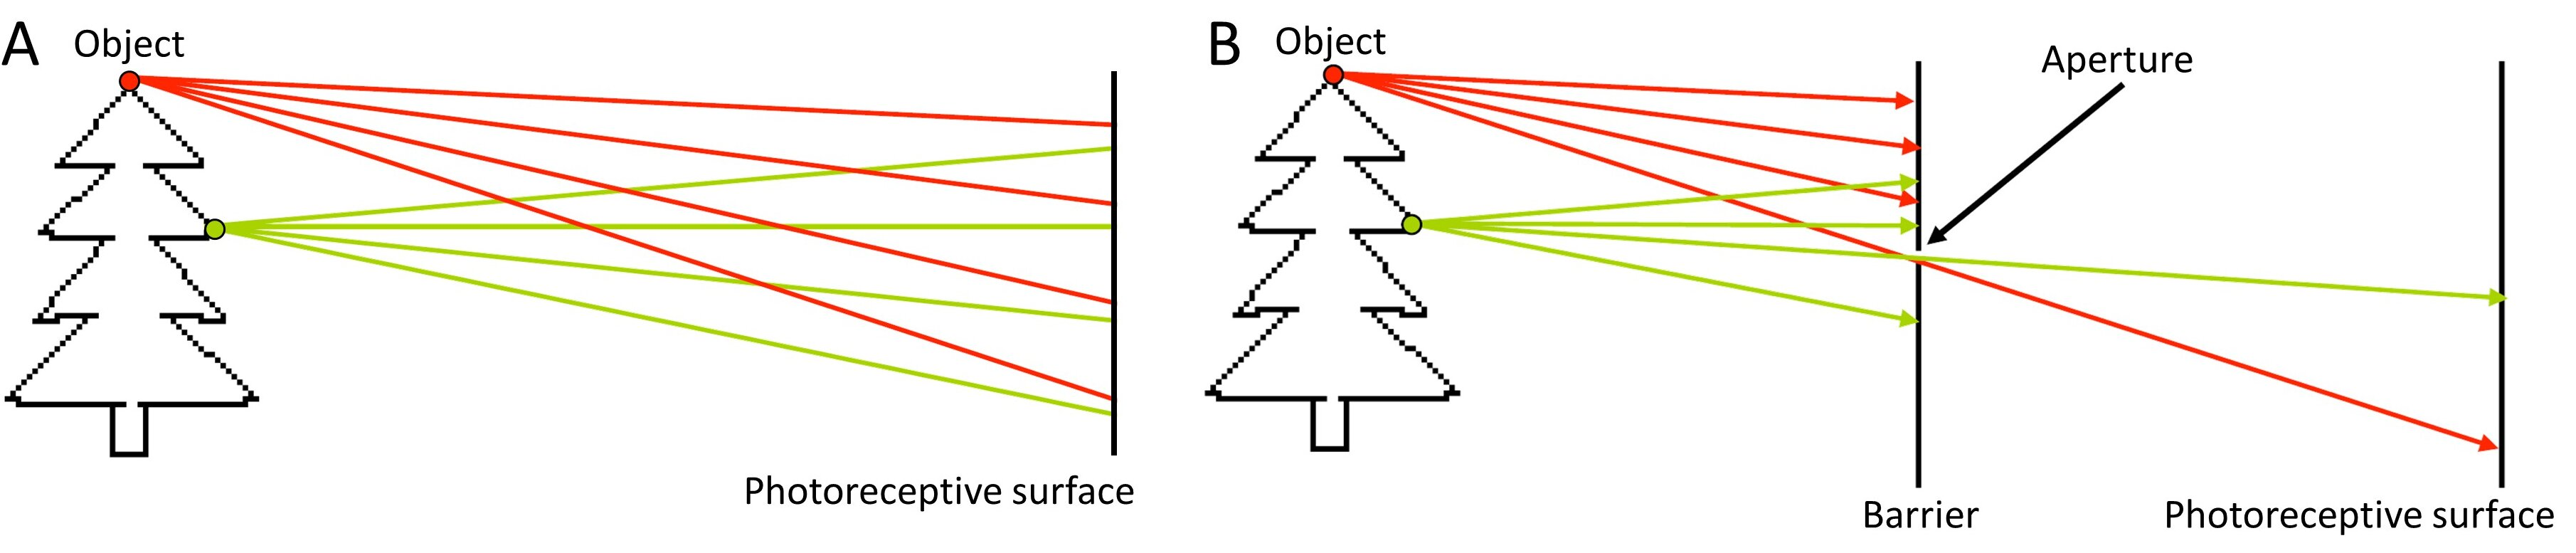
\includegraphics[width=\textwidth]{LightRays0.jpg}
\caption{Light rays on a photoreceptive surface referred to as the image plane. In (A), the image is blurry whereas in (B), a barrier has been added so that "red" and "green" scattered light rays can be distinguished  \cite{FP}.}
\label{fig:LightRays}
\end{figure}

With this basic model for a camera, the geometry can be described with mathematical equations. First, from viewing Figure \ref{fig:PinholeMath}A, one can see that the object as recorded on the image plane is inverted, so often for mathematical derivations, the virtual image plane is used instead. Next, if we define an origin at the pinhole, $o$, in Figure \ref{fig:PinholeMath}B, we can say that point $P$ on the object has coordinates $(-X,Y,-Z)$, while the point $p$ on the image plane has coordinates $(x,-y,f)$ where $f$ is the focal length. By drawing similar triangles, as the points $P$, $o$, and $p$ are collinear, we can write the following equations where the negative signs cancel when using the virtual image plane:

$$\frac{x}{f}=\frac{X}{Z} \ \ ; \ \  \frac{y}{f}=\frac{Y}{Z}$$

We can then solve for $x$ and $y$ which lie on the image plane and are proportional to pixels coordinates which we will later discuss:

$$x=f\frac{X}{Z} \ \ ; \ \ y=f\frac{Y}{Z}$$

\begin{figure}
\centering
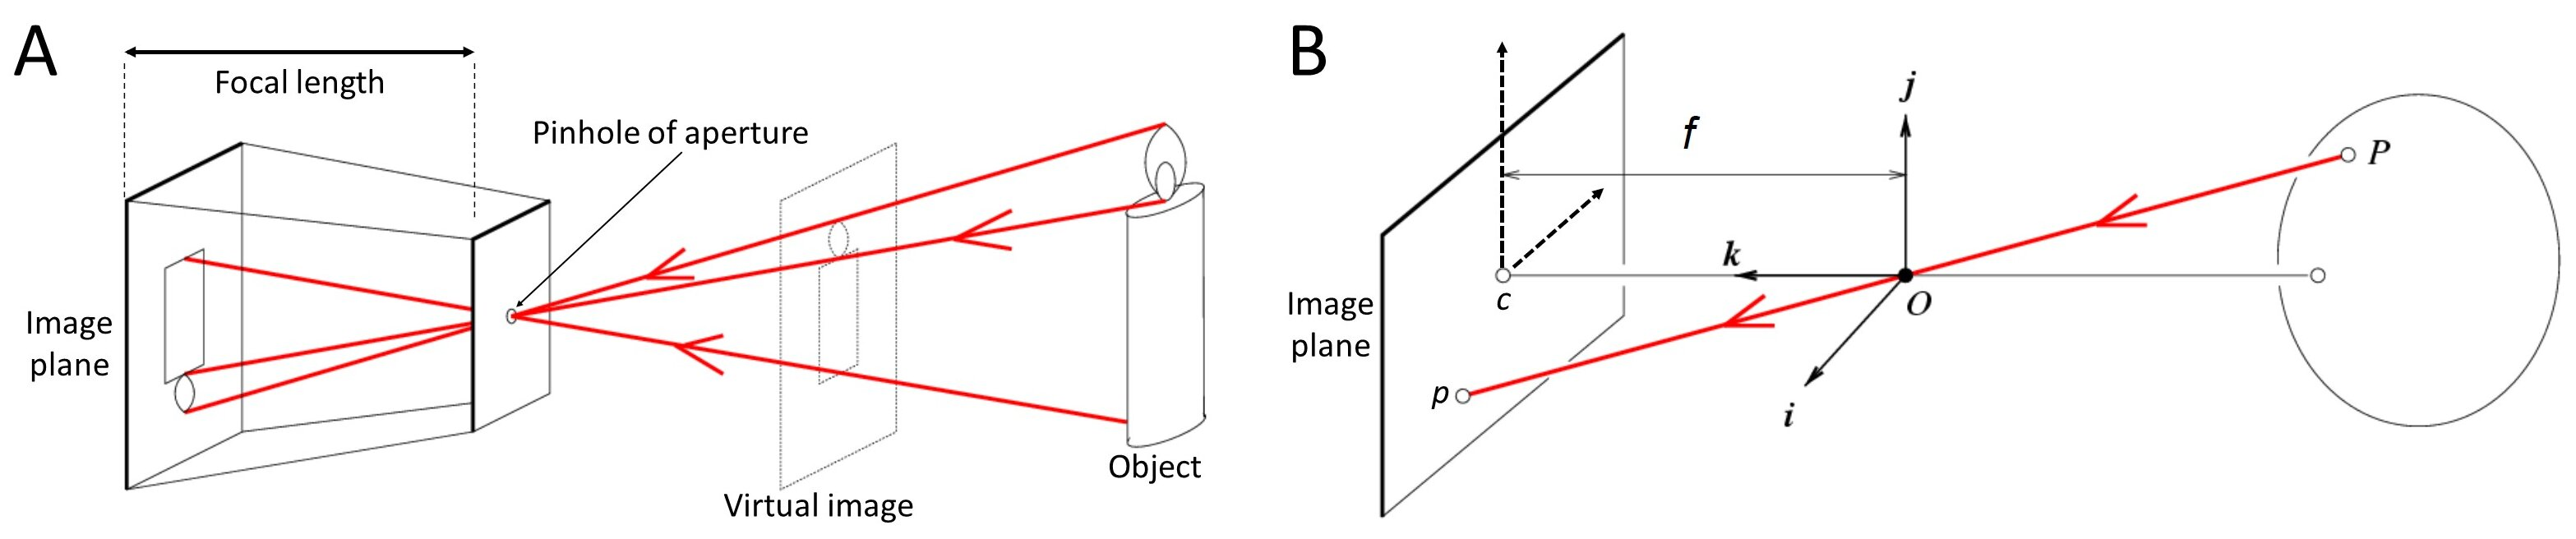
\includegraphics[width=\textwidth]{PinholeMath0.jpg}
\caption{Pinhole camera model. In (A), it can be seen that due to the geometry of the pinhole camera system, the object image is inverted on the image plane and thus, for ease of math, the virtual image plane which displays the non-inverted object is used. In (B), the image center is labeled as $c$, the pinhole is labeled as $o$, the optical axis lies along vector $k$, the focal length is $f$, the 3D point is labeled as $P$, and the 2D pixel point is labeled $p$  \cite{HZ}.}
\label{fig:PinholeMath}
\end{figure}

\subsubsection{Camera lenses}

One limitation of the current pinhole camera model is light. We have already discussed how lacking an aperture, i.e. having an aperture of infinite diameter, leads to a blurry image. But thus far in mathematical terms, we have technically been discussing an aperture of zero diameter which would in reality let in no light. In the middle ground between these two extremes, there is a tradeoff between amount of light that is absorbed by the photoreceptive surface and image blur. Additionally, for small aperture sizes, the resolution becomes fundamentally limited by diffraction in what is called a diffraction-limited system. One clever solution to the lighting-blur issue is to add a lens to replace the aperture as seen in Figure \ref{fig:Lens}A. A lens is an optical element that focuses light by means of refraction. As can be seen however, the light from the object is only focused correctly if the distance to the object equals the focal length of the lens. For any other distance, the image will again appear blurred, although the closer to the focal length distance, the less blur. The size of the 3D region where the blur is acceptably low is called the depth of field.

With this lens, we can now extend our pinhole mathematical model. When looking at Figure \ref{fig:Lens}B, we can use Snell's law and the assumption of a thin lens relative to the focal distance to develop similar triangles. First, rays that pass through the center of the lens are not refracted. Second, rays parallel to the optical axis are focused on the focal point labeled $F'$. Third, all rays passing through point $P$ are focused by the thin lens on the point $p$. Thus, using similar triangles we can write the following equations first using the blue similar triangles then the red similar triangles:

$$\frac{y}{Y}=\frac{z}{Z}=\frac{z-f}{f}$$

Combining these two equations we can write the thin lens equation:

$$\frac{1}{z}+\frac{1}{Z}=\frac{1}{f}$$

We can additionally notice from this geometry that the variable $z$ in the lens model is equivalent to $f$ in the pinhole model and once again notice that points that are not a distance of $Z$ away from the lens will be out of focus. We also see that if $Z$ approaches infinity, light would focus a distance of $f$ away from the lens. Thus, we could assume a pinhole model if the lens is focused at infinity and this could allow us to map 3D points into the camera image plane where they could be converted into pixel coordinates.

\begin{figure}
\centering
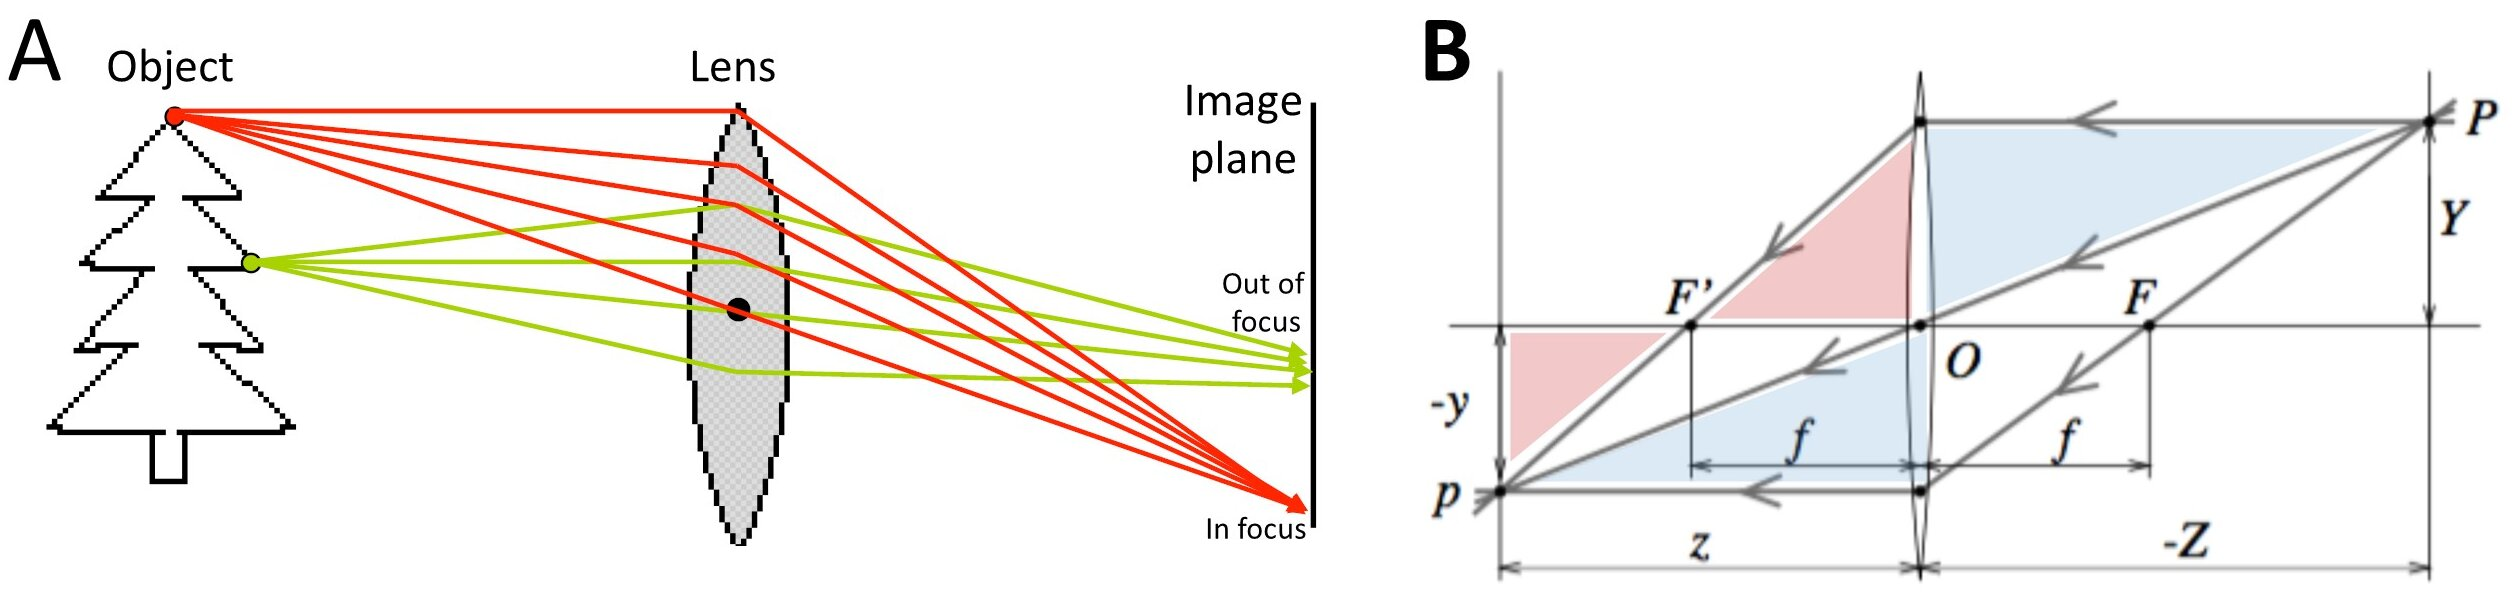
\includegraphics[width=\textwidth]{Lens0.jpg}
\caption{A lens is used to focus light. In (A), a lens is used to focus light originating from an object at a certain distance whereas different distances are blurred. In (B), the thin lens model can be developed using similar triangles  \cite{HZ}.}
\label{fig:Lens}
\end{figure}

\subsubsection{Tradeoffs to optimize light and blur}

With this more complete camera model, we can discuss the tradeoffs involved in most camera applications, especially those involving quickly moving objects, i.e. high-speed cameras. Assuming we want a crisp image without blur, the following factors are critical: object movement, exposure time, receptivity of the photoreceptive surface, aperture size, and lighting conditions. For high speed applications, the exposure time of the camera, or amount of time that the photoreceptive imaging surface absorbs light, needs to be short so that the quickly moving object of interest doesn't move significantly during the exposure time. But with a lower exposure time, less light is absorbed. So to provide more light, we could open the aperture to a larger diameter, but doing so will decrease the depth of field. One solution is to increase the brightness of the light source or sources which is often why extremely bright light sources are used for high speed applications. Regardless, this fundamental issue of light capture exists for cameras especially high-speed cameras, and a proper balance of aperture size and exposure time is needed to optimize blur and image brightness. This, combined with a highly receptive photoreceptive surface and bright lighting conditions need to be considered carefully in photography.


\section{Perspective Projection}
Our goal is \textbf{to determine how points in the world map to points in our camera image}. We start with an assumption of the pinhole camera model (note that all following results also hold when the thin lens model is assumed if we set the camera to be focused at $\infty$ ).

\begin{figure}[H]
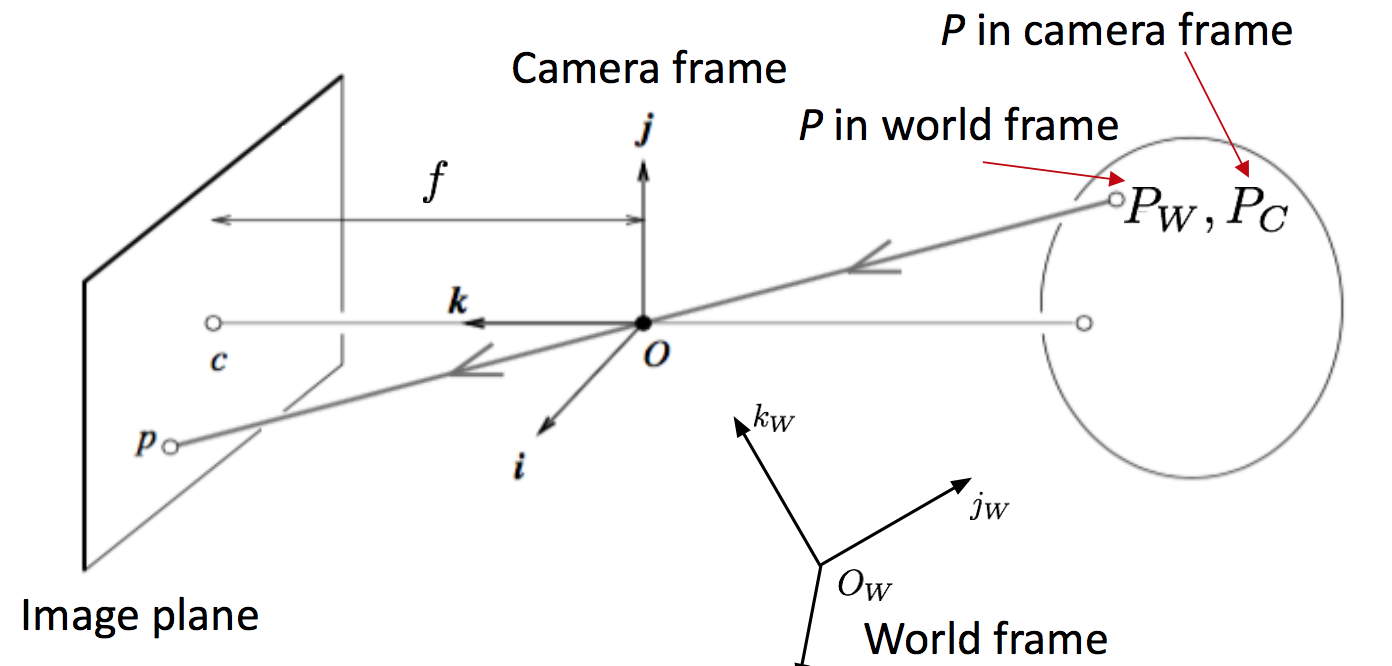
\includegraphics[width=0.4\textwidth]{diagram_1_vik.png}
\centering
\caption{Recall the pinhole camera model discussed in the previous lecture. Our goal is transform coordinates in the world frame $O_w$ to coordinates in the Image Plane. }
\label{fig:pinhole_cam}
\end{figure}

\textbf{Step 1}\\\\
First, we aim to map our point $P_c$ in the camera frame to a point \textit{p} = (\textit{x}, \textit{y}) in the image plane. Recall from the previous lecture:

\begin{center}
\begin{equation}
\begin{tabular}{c}
  $x = f\frac{X_C}{Z_C}$\\
  \\
  $y = f\frac{Y_C}{Z_C}$
\end{tabular}
\end{equation}
\end{center}

Note position of the point in the camera frame, $P_C = [X_C,  Y_C,  Z_c]^T$.

\textbf{Step 2.a}\\\\
Now, we must recognize that the actual origin of a camera coordinate system is not centered on the image plane, but rather usually in the lower right or lower left corner. This is typically done so as to avoid the need for negative coordinates (and consequently, negative array indices) when accessing a specific point on the image plane, which is typically represented as a grid or series of arrays in software.

\begin{figure}[H]
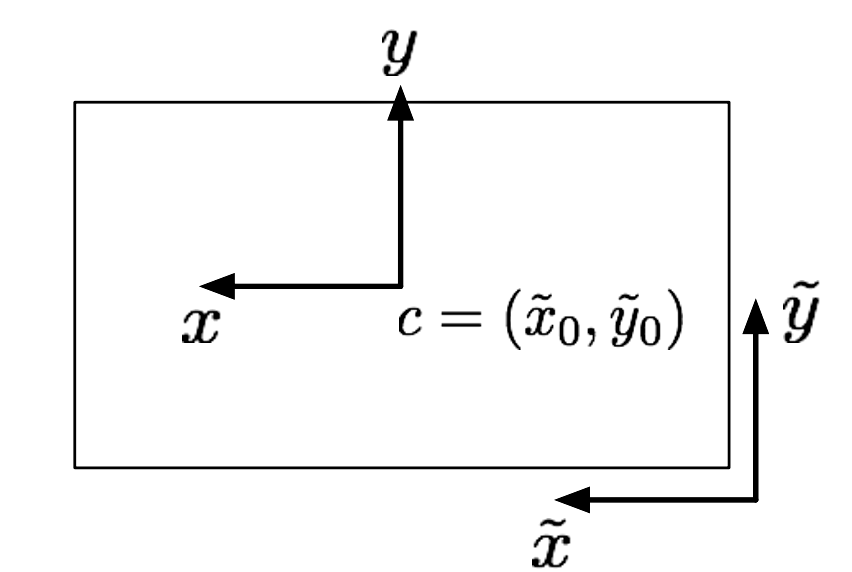
\includegraphics[width=0.4\textwidth]{vik_image_2.png}
\centering
\caption{Here, we place our origin in the lower right corner of the image plane. }
\label{fig:camera_coordinates}
\end{figure}

Given this coordinate translation, it's evident that our old point can be represented in the new axes as:

\begin{center}
\begin{equation}
\begin{tabular}{c}
  $\tilde{x} = f\frac{X_C}{Z_C} + \tilde{x}_0$\\
  \\
  $\tilde{y} = f\frac{Y_C}{Z_C} + \tilde{y}_0$
\end{tabular}
\end{equation}
\end{center}

\textbf{Step 2.b}\\\\
Another issue we must account for is that the ratio of image coordinates to actual pixels is likely not one-to-one. In other words, a shift of one unit in our image plane may correspond to a shift of multiple pixels. Consequently, we introduce $k_x$ and $k_y$ which represent the number of pixels per unit distance in the x and y direction respectively. Although it's certainly possible that $k_x = k_y$, typically this will not be the case if the camera pixels are not square. From this intuition, it follows that:

\begin{center}
\begin{equation}
\begin{tabular}{c}
  $u = k_x\tilde{x} = k_xf\frac{X_C}{Z_C} + k_x\tilde{x}_0$\\
  \\
  $v = k_y\tilde{y} = k_yf\frac{Y_C}{Z_C} + k_y\tilde{y}_0$
\end{tabular}
\end{equation}
\end{center}

We can simplify our result by renaming the following expressions:
\begin{center}
\begin{tabular}{c}
$k_xf = \alpha$\\
\\
$k_yf = \beta$\\
\\
$k_x\tilde{x}_0 = u_0$\\
\\
$k_y\tilde{y}_0 = v_0$
\end{tabular}
\end{center}

Giving us a final result of:

\begin{center}
\begin{equation}
\begin{tabular}{c}
  $u = \alpha\frac{X_C}{Z_C} + u_0$\\
  \\
  $v = \beta\frac{Y_C}{Z_C} + v_0$
\end{tabular}
\end{equation}
\end{center}

\textbf{Homogeneous Coordinates}\\\\
We now note that our transformations from camera frame to pixel value are, unfortunately, not linear. If we can represent these transformations as a linear mapping, we will be able to greatly simplify our math later on. Thus, we introduce the idea of homogeneous coordinates. For a point ($x$, $y$), the homogeneous coordinates ($x_1$, $x_2$, $x_3$) are defined for any three points such that  $\frac{x_1}{x_3} = x$ and $\frac{x_2}{x_3} = y$. \\\\ Consequently, we use the following rules to transform from inhomogeneous coordinates to homogeneous ones. A two-dimensional position, ($x$,$y$) gains a third dimension while a three-dimensional position, ($x$,$y$,$z$) gains a fourth-dimension as a homogeneous coordinate.\\\\


\begin{center}
$\begin{pmatrix}
x \\
y \\
\end{pmatrix}
$
$\Rightarrow$
$\lambda\begin{pmatrix}
x \\
y \\
1
\end{pmatrix}
$
and
$\begin{pmatrix}
x \\
y \\
z
\end{pmatrix}
$
$\Rightarrow$
$\lambda\begin{pmatrix}
x \\
y \\
z \\
1
\end{pmatrix}
$
\end{center}
Similarly, we use these rules to transform back from homogeneous coordinates to inhomogeneous ones. \\\\
\begin{center}
$\lambda\begin{pmatrix}
x \\
y \\
w
\end{pmatrix}
$
$\Rightarrow$
$\begin{pmatrix}
x/w \\
y/w \\
\end{pmatrix}
$
and
$\lambda\begin{pmatrix}
x \\
y \\
z \\
w
\end{pmatrix}
$
$\Rightarrow$
$\begin{pmatrix}
x/w \\
y/w \\
z/w
\end{pmatrix}
$
\end{center}
Note that as we continue to use homogeneous coordinates, we might signal that a specific coordinate matrix is in homogeneous form by using a superscript $h$ (e.g. $P^h$).



%%%%%% Beginning of Lucy's Section %%%%%%%%%
\section{Perspective Projection In Homogeneous Coordinates}

When we shift to representing our points in homogeneous coordinates, we arrive at the following result; note that this is equivalent to the set of equations we derived earlier which translated $P_C$ to the Image Plane, but now $P_C$ is homogeneous.
\begin{equation}
\begin{bmatrix}
\alpha & 0 & u_{0} & 0 \\
0 & \beta & v_{0} & 0  \\
0 & 0 & 1 & 0
\end{bmatrix}
\begin{pmatrix}
X_{c} \\
Y_{c} \\
Z_{c} \\
1
\end{pmatrix}
=
\begin{pmatrix}
\alpha X_{c} + u_{0}Z_{c} \\
\beta Y_{c} + v_{0}Z_{c} \\
Z_{c} \\
\end{pmatrix}
\end{equation}
$\begin{pmatrix}
X_{c} \\
Y_{c} \\
Z_{c} \\
1
\end{pmatrix}
$
is our pixel $P_C$ in homogeneous coordinates; we will ultimately map these coordinates to $P_W$ or world coordinates.
The preceding 3x4 matrix is called $K$, and is alternatively referred to as the camera matrix or matrix of intrinsic parameters. $K$ contains the fundamental characteristics of our given pinhole camera. Although we may have access to these values from the manufacturer specs, we often have to re-calibrate the camera to account for differences in tolerances or noise.

The $K$ depicted in the above equation is typically standard. However, in some rare cases, the Image Plane coordinate axes may not be perpendicular, forcing us to introduce another variable, $\gamma$, representing this skew parameter Typically, we treat $\gamma$ as 0.
\begin{equation}
K =
\begin{bmatrix}
\alpha & \gamma & u_{0} & 0 \\
0 & \beta & v_{0} & 0  \\
0 & 0 & 1 & 0
\end{bmatrix}
\end{equation}
Now, our next step is mapping between the world frame and digital camera frame.

\begin{figure}[H]
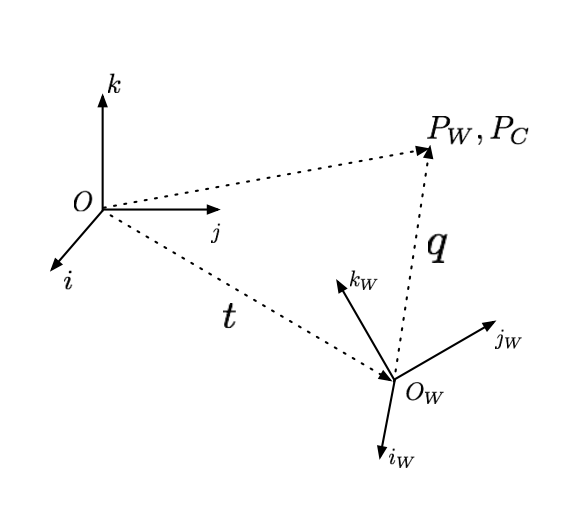
\includegraphics[width=0.4\textwidth]{vik_image_3.png}
\centering
\caption{Here, we depict our point ($P_W$ or $P_C$) relative to the origins of the camera frame and world frame ($O$ and $O_W$ respectively). }
\label{fig:camera_coordinates}
\end{figure}

From this depiction, we have the following:
\begin{equation}
\label{eq:ising}
P_{C} = t + q
\end{equation}
We express $P$ in the camera reference through vector addition. $t$ is the vector from the origin of camera frame to the origin of the world frame. $q$ is the vector representing the position of $P$ with respect to the world frame.\\\\
How do we determine $q$ in relation to the camera frame instead of the world frame? We say:
\begin{equation}
\label{eq:ising}
q = RP_{w}
\end{equation}
where R is the rotation matrix relating camera frame to world frame. Now, we must determine $R$. We start by re-expressing our vector $q$, as seen below:
\begin{equation}
\label{eq:1}
q = q_{x,c} \cdot \hat{i} + q_{y,c} \cdot \hat{j} + q_{z,c} \cdot \hat{k}
\end{equation}
The above equation expresses q with relation to the camera frame.
At the same time, $q$ can also be expressed with respect to the world frame:
\begin{equation}
\label{eq:ising}
q = q_{x,w} \cdot \hat{i_{w}} + q_{y,w} \cdot \hat{j_{w}} + q_{z,w} \cdot \hat{k_{w}}
\end{equation}

We know these two expressions refer to the same $q$, so:
\begin{equation}
\label{eq:ising}
q_{x,w} \cdot \hat{i_{w}} + q_{y,w} \cdot \hat{j_{w}} + q_{z,w} \cdot \hat{k_{w}} = q_{x,c} \cdot \hat{i} + q_{y,c} \cdot \hat{j} + q_{z,c} \cdot \hat{k}
\end{equation}

Now, for example, we might take the dot product of both sides with the unit vector $\hat{i}$. Because the dot product of orthogonal vectors is 0, we are able to eliminate some terms and are left with the following:
\begin{equation}
q_{x,c} = q_{x,w}\hat{i_w} \cdot \hat{i} + q_{y,w}\hat{j_w} \cdot \hat{i} + q_{z,w}\hat{k_w} \cdot \hat{i}
\end{equation}\\
The derivation of the the other coordinates between world and camera frame is similar, and we get the following rotation matrix:

\begin{equation}
R =
\begin{bmatrix}
\hat{i_w} \cdot \hat{i} & \hat{j_w} \cdot \hat{i} & \hat{k_w} \cdot \hat{i} \\
\hat{i_w} \cdot \hat{j} & \hat{j_w} \cdot \hat{j} & \hat{k_w} \cdot \hat{j} \\
\hat{i_w} \cdot \hat{k} & \hat{j_w} \cdot \hat{k} & \hat{k_w} \cdot \hat{k}
\end{bmatrix}
\end{equation}

These sorts of matrices are common in image processing and camera-related tasks.

%%%%%%% Beginning of Nathan's Section
\section{Finalizing the Transformation}
We are able to express the rigid transformation containing both rotation and translation between a point in the world frame to a point in the camera frame by using homogeneous coordinates as follows:

\begin{equation}
\begin{bmatrix}
P_c \\
1
\end{bmatrix}
=
\begin{bmatrix}
R && t \\
0_{3x0} && 1
\end{bmatrix}
\begin{bmatrix}
P_w \\ 1
\end{bmatrix}
\end{equation}

We can combine the transform between a point in the world frame to a point in the camera frame and the transform from a point in the camera frame to a point in the image frame to generate the transform from the the world frame directly to the image frame:

 \begin{equation}
p^h
=
K \begin{bmatrix}
I_{3x3} \quad 0_{3x1}
\end{bmatrix}
\begin{bmatrix}
R && t \\
0_{3x0} && 1
\end{bmatrix}
P_w^h
 \end{equation}

 \begin{equation}
 p^h = K[R \quad t] P_W^h.
 \end{equation}

Here the matrix $K$ is the matrix of intrinsic parameters, and the $[R \quad t]$ matrix contains the extrinsic parameters, which describe the cameras relationship to the points in the photograph. The superscript $h$ means the point is expressed in homogeneous coordinates, meaning that $p^h$ is the $3x1$ homogeneous coordinates matrix of the point in the image frame, and $P_w^h$ is the $4x1$ homogeneous coordinates matrix of the point in the world frame.

The total degrees of freedom for the combined matrices are 5 for $K$, 3 for the rotation matrix $R$ and 3 for the translation $t$, leading to a total of 11 parameters. Note that the rotation matrix $R$ has 3 DOF because rotation of a coordinate frame takes place in three linearly independent planes. If we assume that our skewness $\gamma$ is 0, K has 4 parameters and the total number of degrees of freedom is 10 instead.

This perspective projection naturally causes several consequences which can be mathematically derived. For example, parallel lines in images appear to meet at the horizon, and objects that are far away appear smaller than their closer counterparts. Both effects are shown in the following image of train tracks.

\begin{figure}[H]
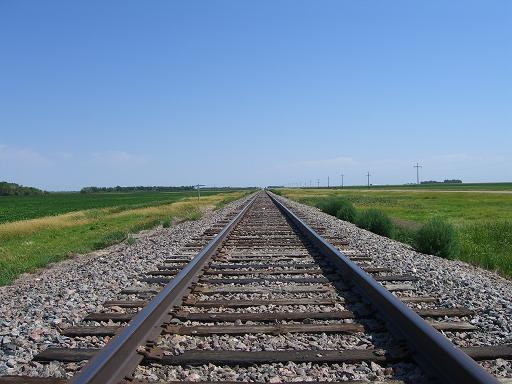
\includegraphics[width=0.5\textwidth]{traintracks.jpg}
\centering
\caption{An image of train tracks. Note that the parallel tracks appear to meet at the horizon. The wooden railroad ties (perpendicular to the tracks) are all the same size, but those further from the camera appear smaller than the closer railroad ties. }
\label{fig:train_tracks}
\end{figure}


\subsection{Direct Linear Calibration}
The problem of direct linear calibration is the following: given known correspondences between known points in the camera frame $(p_i)$ and known points in the world frame $P_{W,i}$, determine the intrinsic parameters $(K)$ and the extrinsic parameters $(R,t)$ of the camera.

A common method of determining these known correspondences is to use images of a grid with a chessboard like pattern. Such a pattern enables simple extraction of the corners, and identification of relationships between objects in the world frame.

%%%%%%%% Beginning of Huajian's Section
\section{Solving Calibration Problems}

The major idea in camera calibration is that, given some known positions in the image frame, and the corresponding world frame positions, we back out the components of the matrices in the previous sections. These matrices include (1) the intrinsic parameter matrix, (2) the rotation matrix from image frame to world frame, and (3) the vector connecting the world frame and image frame.\\

\begin{figure}[H]
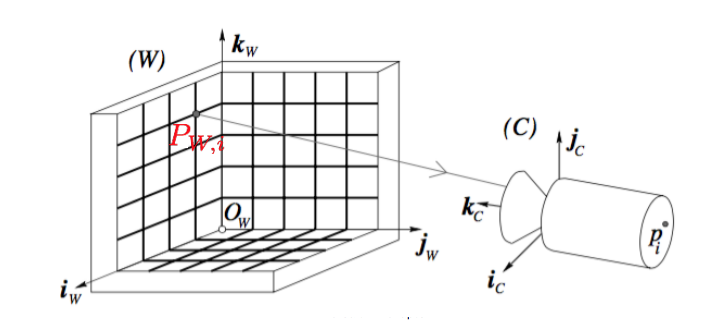
\includegraphics[width=0.5\textwidth]{vik_image_4.png}
\centering
\caption{An example of camera calibration. Here, we know the relationship between the red point $P_{W,i}$ in the world and $p_i$ in the image plane.}
\label{fig:calibration}
\end{figure}


First of all, we have the fundamental relationships, relating $p_i^h$, the projected point on the image plane in homogeneous coordinates, and $P_{W,i}^h$ the corresponding point in the world frame in homogeneous coordinates:
\begin{equation}
    p_i^h = M P_{W,i}^{h}\hspace{1mm}, \hspace{3mm}i = 1,....n
\end{equation}

where
\begin{equation}
    M = K [R \hspace{2mm} t]=
\begin{bmatrix}
    m_1 \\
    m_2 \\
    m_3
\end{bmatrix}
\end{equation}




The process involves feeding in $n$ corresponding pairs of image frame positions and world frame positions, where $i$ is the index of the current pair. The $M$ matrix is size 3 by 4, and each $m_i$ is size 1 by 4. Note that we are working with homogeneous coordinates. We have:
\begin{equation}
    p_i^h = [\lambda u \hspace{2mm} \lambda v \hspace{2mm} \lambda]^T
\end{equation}
\begin{equation}
        P_{W,i}^{h} = [x \hspace{2mm} y \hspace{2mm} z \hspace{2mm} 1]^T
\end{equation}
which conforms with the matrix multiplication rules given $M$ is 3 by 4.\\


If we write out the relationships between a pair of $p_i^h$ and $P_{W,i}^h$, we can obtain the following:
\begin{equation}
    \lambda = m_3 \cdot P_{W,i}^h
\end{equation}

\begin{equation}
    u_i = \frac{\lambda u_i}{\lambda} = \frac{m_1 \cdot P_{W,i}^h}{m_3 \cdot P_{W,i}^h}
\end{equation}
\begin{equation}
    v_i = \frac{\lambda v_i}{\lambda} = \frac{m_2 \cdot P_{W,i}^h}{m_3 \cdot P_{W,i}^h}
\end{equation}

which can be transformed into the form of two constraint equations:
\begin{equation}\label{eqn:u_contraint}
    u_i(m_3 \cdot P_{W,i}^h) - m_1 \cdot P_{W,i}^h = 0
\end{equation}
\begin{equation}
    v_i(m_3 \cdot P_{W,i}^h) - m_2 \cdot P_{W,i}^h = 0
\end{equation}

Now if we stack all of these (n pairs of these $u_i$ and $v_i$ equations) together, we can obtain a system of equations, and to write them compactly, we can use matrix multiplication:
\begin{equation}
    \tilde{P}m = 0, \hspace{5mm} m =
    \begin{bmatrix}
    m_1^T \\
    m_2^T \\
    m_3^T
\end{bmatrix}
\end{equation}

Let's write out a few rows of $\tilde{P}$ that correspond to the $u_i$ and $v_i$ constraints above to make things more concrete:


\begin{equation}
\tilde{P} =
     \begin{bmatrix}
  -(P_{W,1}^h)^T & 0_{1x4} & u_{1} (P_{W,1}^h)^T \\
   0_{1x4} & -(P_{W,1}^h)^T &v_{1} (P_{W,1}^h)^T  \\
  -(P_{W,2}^h)^T & 0_{1x4} & u_{2} (P_{W,2}^h)^T \\
  \vdots & \vdots & \vdots
 \end{bmatrix}
\end{equation}



The size of $\tilde{P}$ is 2n by 12, and the size of $m$ is 12 by 1.


Now, we ideally want to directly solve this system of equations and obtain the unique set of $m_i$ values, which should allow us to obtain all parameters of the camera. We have 12 parameters to determine (including the scaling parameter for the projection). Potentially, we might want to feed in more pairs of corresponding positions to make this process more robust; however, that would result in more equations than coefficients to solve for, making the problem "over-constrained". \\\\
Furthermore, due to the uncertainties which arise in obtaining any of these positions data, it's very likely that this system of equations is not perfectly satisfied. Therefore, we will frame this as a minimization problem where we try to satisfy this system of equations as well as possible, with a non-trivial $m$ coefficient vector. Note that, without the constraint of square norm of $m$ equals 1, the minimization would result in trivial coefficients (all $m_i$ being zeros).

\begin{equation}
    min_{m\in R^{12}} \hspace{3mm} \| \tilde{P} m \|^2
\end{equation}
subject to
\begin{equation}
    \| m \|^2 = 1
\end{equation}

This choice of the norm of $m$ relies on the fact the a scalar multiple of the solution is still a solution of the original system of equations. Now, let's construct the Lagrangian first, by adding the cost and the Lagrange multiplier times the constraint:
\begin{equation}
    L = m^T\tilde{P}^T\tilde{P}m + \lambda(1 - m^T m)
\end{equation}
We take the gradient and set it to zero as the necessary condition of optimality:
\begin{equation}
    \nabla L = 2\tilde{P}^T \tilde{P} m - 2\lambda m = 0  \xrightarrow{} \tilde{P}^T \tilde{P} m = \lambda m
\end{equation}

Now, it's obvious that the $m$ we are looking for is an eigenvector of the $\tilde{P}^T \tilde{P}$. Furthermore, it is the eigenvector that has the smallest eigenvalue that would minimize the square norm.


After obtaining the $M$ matrix upon solving the minimization problem, we will factorize $M$ as
\begin{equation}
    M = [KR \hspace{2mm} Kt]
\end{equation}
The first 3 columns of the matrix are the product of the intrinsic parameter matrix, which is upper triangular, and the rotation matrix, which is orthogonal. This calls for the efficient RQ factorization method, and we can obtain the parameters from the corresponding entries.


%%%%%%% Beginning of Zaifeng's Section

\section{Radial Distortion}
So far, there's another problem not being considered: radial distortion. For a real lens, the linear assumption will not hold any more. Either barrel distortion or pincushion distortion will exist and affect the real pixel coordinates.

\begin{figure}[H]
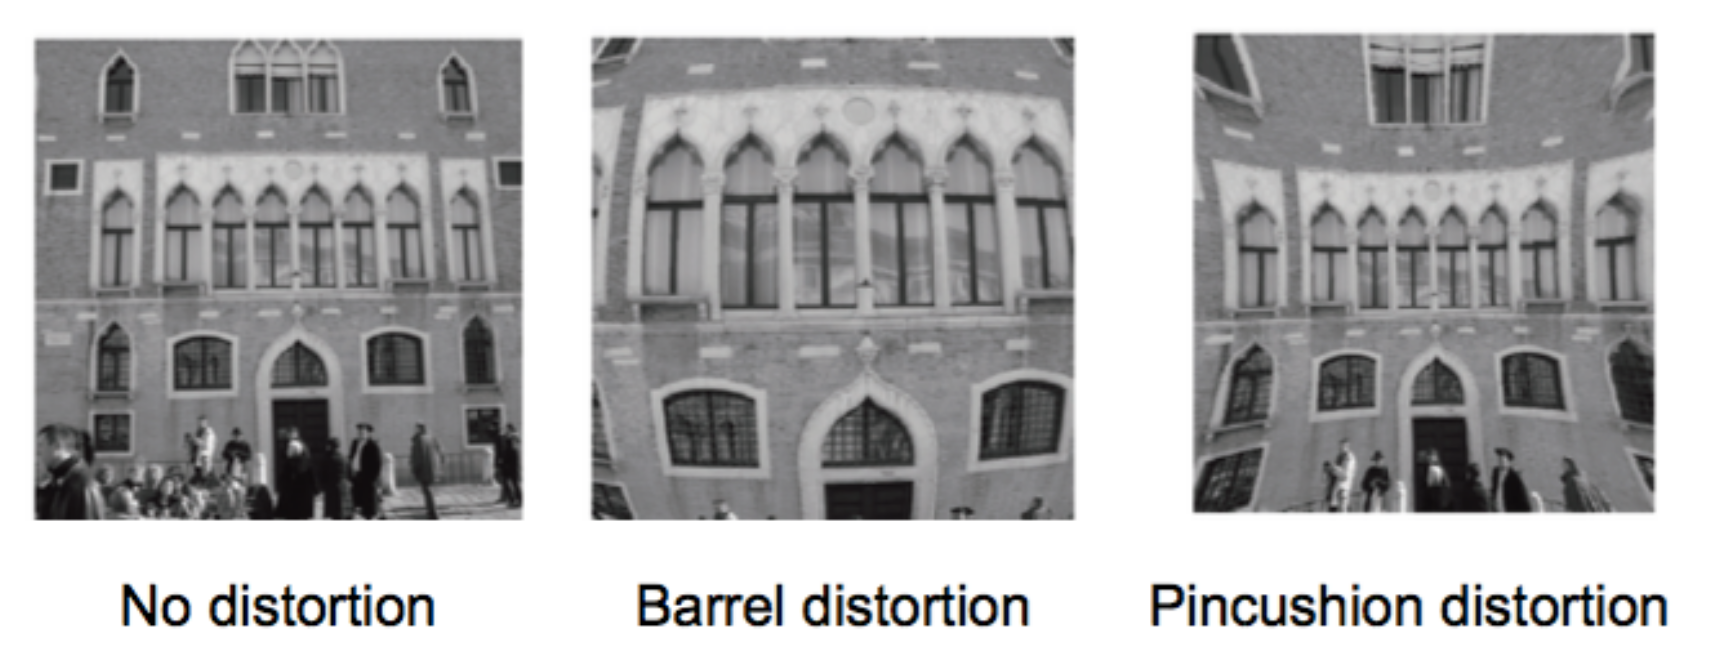
\includegraphics[width=0.5\textwidth]{distortion.png}
\centering
\caption{Different kinds of distortions}
\label{fig:distortion}
\end{figure}

There are many algorithms that address image distortion. A simple and efficient way is to set up relations between the ideal pixel position $(u,v)$ and the distorted pixel position $(u_d,v_d)$

\begin{equation}
\begin{bmatrix}
    u_d \\
    v_d
\end{bmatrix}
=
\begin{bmatrix}
    u_d \\
    v_d
\end{bmatrix}
(1+kr^2)
\begin{bmatrix}
    u-u_{cd} \\
    v-v_{cd}
\end{bmatrix}
+
\begin{bmatrix}
    u_{cd} \\
    v_{cd}
\end{bmatrix}
\end{equation}

where $k$ is the radial distortion factor that differs in different cameras and needs to be pre-calculated. $r^2=(u-u_{cd})^2+(v-v_{cd})^2$ is the square of the distance between the ideal pixel location and the center of distortion. $(u_{cd},v_{cd})$ are the coordinates of the image center.

Although this algorithm is efficient, there are many more sophisticated tools which we will not address.

\section{Measuring Depth}
Now, once we know our parameters $K,R,t$, can we find out the corresponding coordinates in the real world if $p$ on our image plane is known?

Unfortunately, the answer is no. That's because the equation $p^h=K[R t]P_W^h$ is not revertible. We still need to decide an extra variable in the 3D world - the depth of $P$, $Z_W$. The only thing we are sure now is that P lies along the line connecting $O$ and $p$.

\begin{figure}[H]
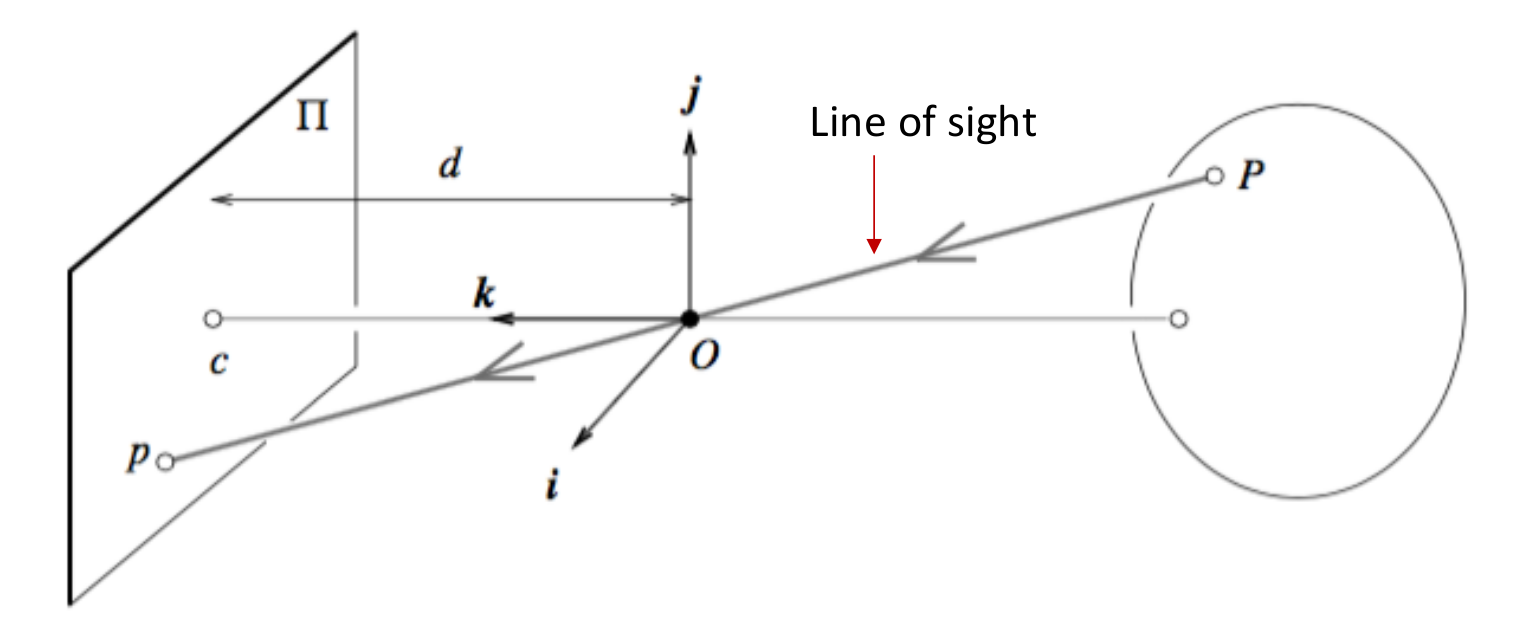
\includegraphics[width=0.3\textwidth]{measuring_depth.png}
\centering
\caption{The depth of the real object is not known yet.}
\label{fig:measuring_depth}
\end{figure}

\section{Recovering Structure}
The previous discussion tells us that we can not simply determine the depth/structure from the pixel coordinates and camera parameters. We see this effect when we look at the picture below. We only know the man is not really stepping on the tower because of our own contextual clues or experience, not from the picture itself.

\begin{figure}[H]
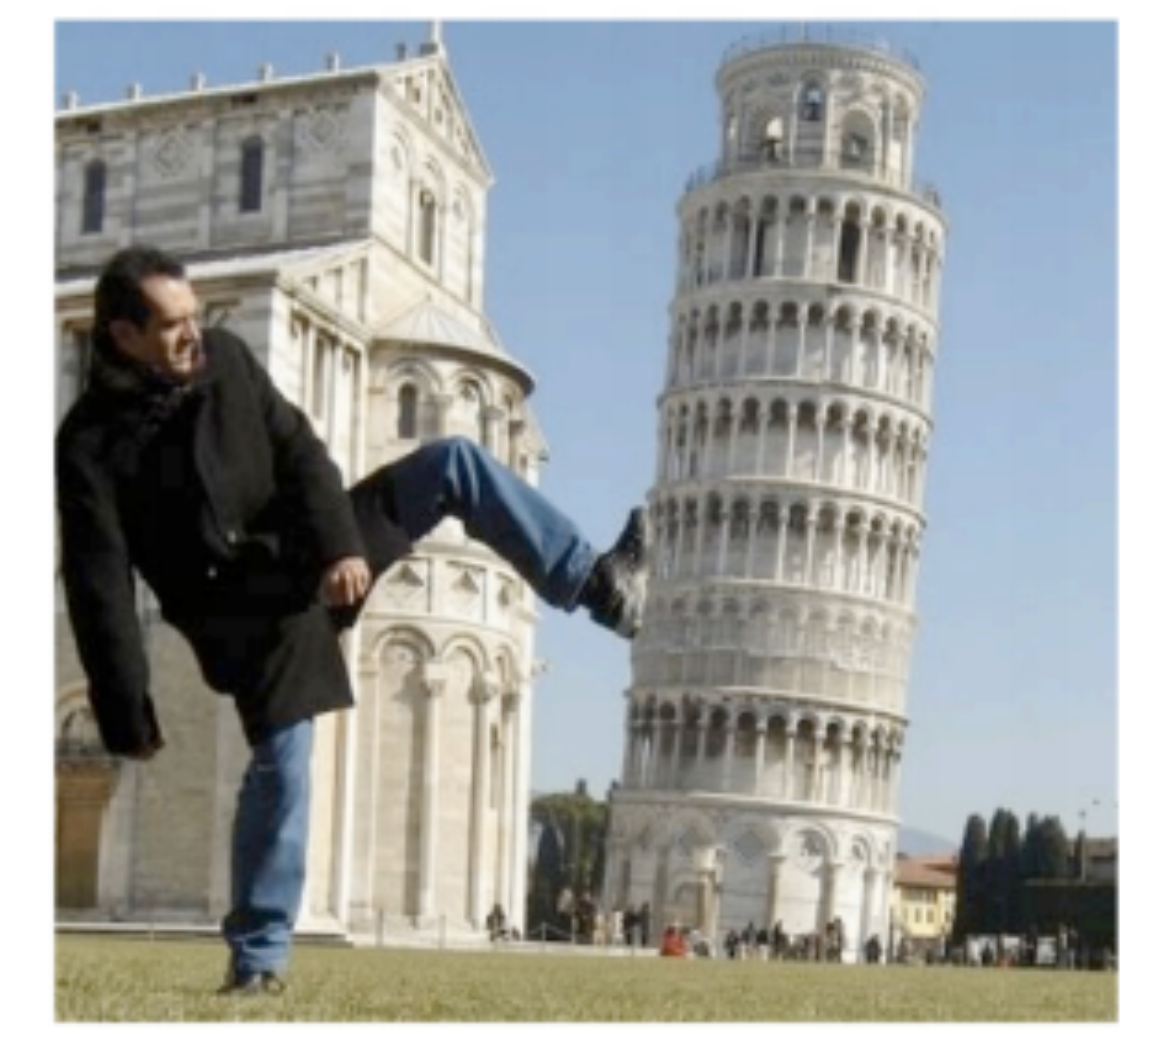
\includegraphics[width=0.3\textwidth]{stepping_on_tower.png}
\centering
\caption{In the picture, the man seems to be stepping on the tower.}
\label{fig:stepping_on_tower}
\end{figure}

However, we can achieve the goal using other tools. This process is usually called structure recovering - we aim to reconstruct a 3D scene only with access to 2D images. Some common methods are listed below.

\begin{itemize}
  \item Through	recognition of landmarks (e.g., orthogonal walls)
  \item Depth from focus: determines distance to one point by taking multiple images with better and better focus
  \item Stereo vision: processes two distinct images taken at the same time and assumes that the relative pose between the two cameras is known
  \item Structure from motion: processes two images taken with the same or different cameras at different times and from different unknown positions
\end{itemize}


%% TODO: move these references to the bib file, and add citations within the body.
\section{References}
Relevant readings related to or referenced in the lecture include:
\begin{itemize}
  \item SNS: 4.2.3
  \item D.A.Forsyth	and	J.	Ponce[FP]. Computer Vision:	A	Modern	Approach	(2nd
Edition).	Prentice	Hall,	2011.	Chapter	1.
  \item R.	Hartley	and	A.	Zisserman	[HZ].	Multiple	View	Geometry	in	Computer
Vision.	Academic	Press,	2002.	Chapter	6.1.
  \item Z.	Zhang.	A	Flexible	New	Technique	for	Camera	Calibration. IEEE	Transactions
on	Pattern	Analysis	and	Machine	Intelligence,	2000.
\end{itemize}

\bibliographystyle{unsrt}%Used BibTeX style is unsrt
\bibliography{reference}


\subsubsection*{Contributors}
Winter 2019: [Your Names Here]
\\
Winter 2018: Nathan Usevitch, Vik Pattabi, Huajian Huang, Zaifeng Zheng, Lucy Zhuang

\end{document}
